\documentclass[10pt, a4paper,twocolumn]{article}
\usepackage[latin1]{inputenc}
\usepackage{amsmath}
\usepackage{amsfonts}
\usepackage{amssymb}
\usepackage{graphicx}
\usepackage{xcolor}
\usepackage{hyperref}
\usepackage{booktabs}
\usepackage[normalem]{ulem}


\newcommand\hl{\bgroup\markoverwith
	{\textcolor{yellow}{\rule[-.5ex]{.1pt}{2.5ex}}}\ULon}


\title{Toxic Comment Classification - Report}

\author{Mick van Hulst \and Dennis Verheijen \and Roel van der burg \and Brian Westerweel \and Joost Besseling}

\begin{document}
	\maketitle
	
	\section{Problem statement}
	We have chosen the toxic comment classification challenge on Kaggle. For this challenge we have to classify about 160000 comment. There are 6 different classes and each comment can be labeled with any of these classes. This means our problem is a multilabel classification problem.
	
	\section{Dataset}
	
	The dataset that is provided by Kaggle consists of some 160000 comments with their respective class labels. They also provide a test set of about the same size, without the labels. Our task is to predict the labels of the test set.
	%TODO een voorbeeld sample
	
	One important characteristic of our data is that the set is very imbalanced (figure \ref{fig:imbalance}). This posed many challenges to us.
	
	\begin{figure}[h]
		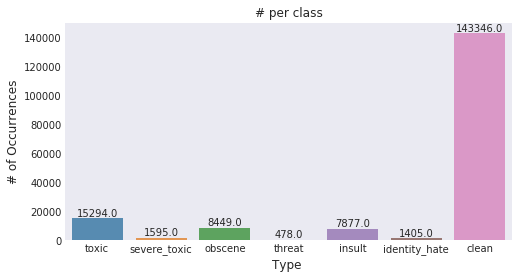
\includegraphics[width=0.4\textwidth]{img/distribution_histogram}
		\caption{Figure from Kaggle \cite{abc}}
		\label{fig:imbalance}
	\end{figure}
	
	
	\subsection*{Data Preprocessing}
	Since the data consists of raw Wikipedia comments, we have to do some preprocessing to convert the words to lowercase and change words that are spelled erroneously to the correct spelling. We use the TweetTokenizer to handle this for us.
	
	\begin{table*}[t]
		\centering
		\begin{tabular}{l|c}
			\toprule
			\textbf{Method} & \textbf{AUC} \\
			\midrule
			Feature Based Approach v1 & 0.59 \\
			Feature Based Approach v2 & TBA \\
			Convolutional Neural Network & 0.4902 \\
			Vanilla LSTM & TBA \\
			Biirectional LSTM & 0.96 \\
			\bottomrule
		\end{tabular}
		\caption{Summary of the achieved results, the Area Under the Curve (AUC) are computed using Kaggle.}
		\label{table:summary_results}
	\end{table*}
	
	
	\section{Models}
	In this section, the different approaches will be described. Starting with feature extraction, followed by Neural Network approaches including language modeling with an LSTM and a convolutional approach.
	
	\subsection{Feature Extraction}
	The first approach that was used was feature extraction. The goal was to extract meaningful features from the text to classify samples separately per class. The features were handcrafted, such that they are tangible features (i.e. not generated by a Neural Network).
	\subsubsection{Feature Based Approach v1}
	In the first iteration of this approach, more generic features were used:
	\begin{itemize}
		\setlength\itemsep{0px}
		\item Ratio of capitals vs total characters
		\item Ratio of punctuation characters
		\item Total length in characters, words and in sentences
		\item Total amount of some special characters: ?, (, ), ! and some other characters.
		\item Amount of unique words		
	\end{itemize}
	In total, about ten features were generated. These features were used to train various classifiers, which will be described in section \ref{sec:classifiers}. Each model was evaluated separately. However, as may be noted from the results but in the end, none of these feature based models managed to produce convincing results.
	
	
	\subsubsection{Feature Based Approach v2}
	
	After a meeting with our supervisor, we thought that a problem with our feature extraction was that we might be using too little features. Since we are trying to predict 6 classes separately, and we are using a quite complex set, the dimensionality of the set is probably higher than 10. That is why we decided to introduce some extra features.
	
	\begin{itemize}
		\item For a list of swear words (since we are doing \emph{toxic} comment classification), we added a feature denoting whether that particular word occurred in the comment.
		\item {\color{red}More features??} 
	\end{itemize}
	
	This greatly improved our results.

	\subsubsection{Classifiers}
	\label{sec:classifiers}
%	\subsubsection*{MultiLayer Perceptrons}
	\textbf{Multilayer Perceptrons}
	The multilater perceptron (MLP) is a very simple neural network, using only fully connected (or dense) layers. In our case, the input consisted of the total number of features, and we used 6 units as output, each denoting the probability that that one of the six respective was active for the current sample. 
	
	We experimented with various configurations of this setup. We varied the number of layers, and the width of the hidden layers.
	
	
	%\subsubsection*{Support Vector Machines}
	\textbf{Support Vector Machines}
	We only used a linear kernel, but the learning time of the SVM was so high, that we quickly decided not to investigate this approach further.
	
%	\subsubsection*{Random Forests}
	\textbf{Random Forests}
	\hl{The random forest classifier also didn't get good results on the small feature set, we have not YET tested it on the big feature set).}
	
% \subsubsection*{1D Convolutional Network}
    \textbf{1D Convolutional Network}
    Another approach we tried is the 1-dimensional convolutional network. However, because this network showed weak results (merely 0.4902 ROC AUC score) we decided to drop this approach.

	\subsection{Neural Networks}
	
	Having implemented these feature based approaches, we decided it might be better to use a neural network model. We decided to use the LSTM (Long Short Term Memory), because LSTM's are recurrent neural networks, so it can learn the context of words in sentences. First we tried to use the most simple LSTM we could think of.
	
	%TODO describe this lstm and its aoc
	
	After that, we found  very well performing LSTM based approach on Kaggle (a bidirectional LSTM). This means that we feed the sentence twice to the LSTM, once normally, from front to back, and once flipped.
	\begin{figure}
	\begin{verbatim}	
	    A forward and backwardsentence
	    sentence backward and forward A
	\end{verbatim}
	\caption{An example of how the  Bidirectional layer would feed the data to the LSTM}
	\end{figure}
	
	
	We implemented a 1 dimensional convolutional neural network.
	
	\section{Data Validation}
	\hl{DO we want to do something in this chapter? It is something we struugled with in the beginning? Maybe it can be merged with the next steps chapter?}
	
	\section{Reflection}
	After the first competition, we have already learned many things. In this section we will briefly discuss a few things that stood out during this competition.
	
	\textbf{Imbalanced dataset:} The one thing that stood out from our dataset is that it was very imbalanced. This made it hard to test if our model was performing correctly as predicting that every comment was non-toxic already resulted in an accuracy of $\approx 0.96$. This made it hard to train our models as during training time the model quickly returned a small loss.
	
	\textbf{Ensemble Methods} During the first competition, we found out that ensemble models are extremely powerful for machine learning tasks (e.g. during the project presentations some groups used these). We have decided that we also want to use ensemble methods in the next competition.
	
	\textbf{Collaboration} After this first project we are more accustomed to each of our group members (i.e. knowing each other's strengths/weaknesses). This makes it easier for us to work together and enables us to divide our tasks accordingly. To efficiently work together, we're going to utilize an existing git strategy, such as git flow. We found great benefits in the weekly meetings and thus we're going to continue doing so.
	\begin{thebibliography}{xx}
		\bibitem{abc}
		\textsc{Jagan}, \textit{Stop the S@\#\$ - Toxic Comments EDA},
		 https://www.kaggle.com/jagangupta/stop-the-s-toxic-comments-eda
	\end{thebibliography}
	
\end{document}